\chapter{Requisiti}
L'obiettivo del progetto è realizzare un \textit{servizio di chat distribuito}. Nella nostra applicazione potranno esserci uno o più \textit{utenti}, i quali potranno unirsi o abbandonare una o più \textit{stanze}. Una stanza è rappresentata da un nome univoco e da un insieme di utenti. All'interno di ogni stanza ogni utente può inviare messaggi altri utenti \textit{partecipanti} e riceverne dagli stessi. L'utente avrà la possibilità di creare e modificare il proprio \textit{profilo} utente e di visualizzare quello dei partecipanti delle stanze in cui è presente. 

\section{Requisiti di business}
Dall'analisi del problema sono emersi i seguenti requisiti funzionali che ci prefiggiamo di implementare:
\begin{itemize}
    \item Possibilità da parte di un utente di \textbf{unirsi a una o più stanze ed abbandonarle}.
    \item \textbf{Eliminazione di una stanza} (solamente da parte del suo creatore).
    \item Possibilità da parte di un utente di \textbf{visualizzare lo stato (effettiva connessione al sistema) degli utenti cha partecipano alla stanza}.
    \item Possibilità di \textbf{visualizzare il profilo utente} (nome utente, nome, biografia, stato).
    \item \textbf{Aggiornamento real-time ai partecipanti di una stanza sullo stato di scrittura} di un utente che digita.
    \item Possibilità di \textbf{cercare una chat per nome}.
    \item Possibilità, da parte di un utente, di \textbf{rendersi invisibile agli altri utenti}.
\end{itemize}
Le funzionalità utente sono state descritti in maniera visuale tramite il diagramma dei casi d'uso in Figura \ref{fig: use-cases}.

\begin{figure}
  \centering
  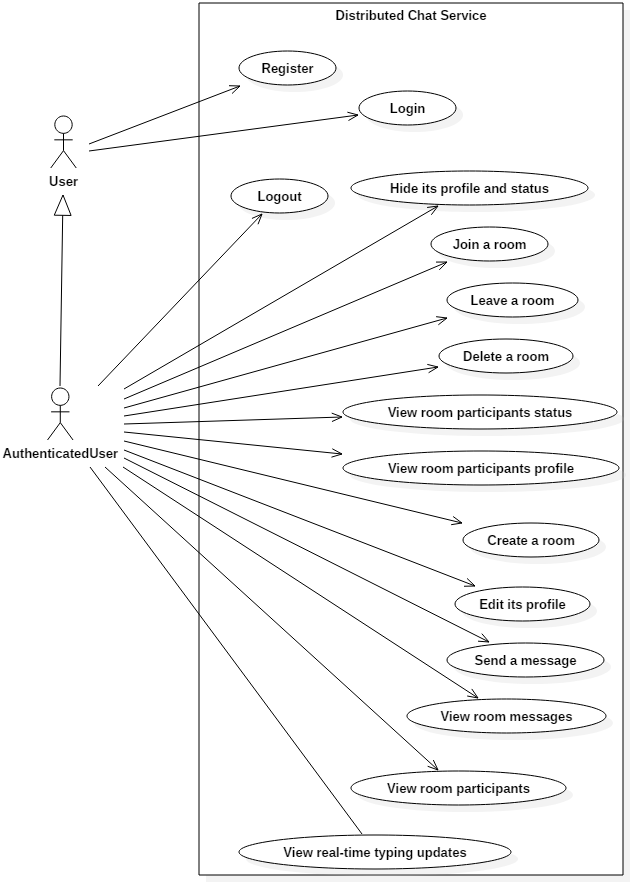
\includegraphics[width=\linewidth, keepaspectratio]{images/UseCaseDiagram.png}
  \caption{Diagramma dei casi d'uso.}
  \label{fig: use-cases}
\end{figure}

\subsection{Unione ad una stanza ed uscita}
L'unione dell'utente ad una stanza comporta la possibilità di visualizzare i messaggi in essa contenuta (anche precedenti al \textit{join} dell'utente), di inviare messaggi e di visualizzare le informazioni sulla stanza (numero, nome e data di join dei partecipanti). È possibile uscire in qualsiasi momento da una stanza a cui ci si era uniti.

\subsection{Eliminazione di una stanza}
È possibile, per il suo creatore, eliminare una stanza indipendentemente dal numero di messaggi e di partecipanti che contiene in un certo momento.

\subsection{Visualizzazione dello stato degli utenti}
Un partecipante ad una stanza può visualizzare lo stato degli altri partecipanti (a meno che lo stato da visualizzare appartenga ad un utente invisibile). Per \textit{stato} si intende l'effettiva \textit{connessione} al servizio di chat in un certo periodo temporale.

\subsection{Visualizzazione e modifica del profilo utente}
Un partecipante ad una stanza può visualizzare il profilo utente degli altri partecipanti (a meno che il profilo da visualizzare appartenga ad un utente invisibile). Il profilo utente è modificabile tramite apposita schermata e comprende: nome utente, nome, biografia e flag di invisibilità. 

\subsection{Aggiornamento real-time sullo stato di scrittura}
Nel momento in cui un utente scrive un messaggio all'interno di una stanza, allora agli utenti che partecipano alla stessa stanza verrà visualizzato il fatto che quell'utente sta digitando.

\subsection{Ricerca di una stanza per nome}
Sarà presente un'apposita schermata di ricerca di una stanza. La ricerca avviene digitando il nome della stanza da trovare.
Nel momento in cui l'utente inizia a digitare, verranno visualizzate tutte le stanze che contengono nel proprio nome la stringa digitata.
Successivamente, sarà possibile effettuare il \textit{join} alla stanza semplicemente cliccando sul suo nome.

\subsection{Offuscamento del proprio stato agli altri utenti}
Tramite la modifica del proprio profilo utente, è possibile impostare un \textit{flag di invisibilità}. Se tale flag è attivo, il proprio profilo ed il proprio stato non saranno visibili da altri utenti. Inoltre, non sarà possibile, per l'utente invisibile, visualizzare lo stato e profilo degli altri utenti.

\section{Requisiti non funzionali}
L'unico requisito non funzionale del sistema è la \textbf{sicurezza del sistema di interazione} tra i componenti del sistema, in particolare del meccanismo di autenticazione. Il sistema di autenticazione dovrà:
    \begin{itemize}
        \item Permettere la registrazione, inserendo \textit{username} e \textit{password}, 	rilasciando un \textit{token} di autenticazione all'utente;
        \item Memorizzare in maniera persistente le informazioni inserite;
        \item Permettere la cancellazione di un utente, fornendo il suo \textit{token} di autenticazione;
        \item Permettere il login, inserendo \textit{username} e \textit{password}, rilasciando un \textit{token} di autenticazione all'utente;
        \item Permettere la validazione di un \textit{token} di autenticazione, ottenendo la descrizione dell'utente in risposta.
    \end{itemize}
\textit{Alcune interazioni (etichettate come protette) tra i componenti del sistema saranno eseguibili soltanto previa autenticazione}; quindi necessiteranno dell'invio, contestuale alla richiesta, di un token precedentemente rilasciato dal sistema di autenticazione.

\section{Requisiti di implementazione}
Per lo sviluppo del progetto sono stati definiti a priori i seguenti requisiti implementativi:

\begin{itemize}
    \item \textbf{Scala}: il linguaggio da utilizzare per lo sviluppo della maggior parte del progetto deve essere \textit{Scala}. Imponiamo questo requisito in quanto vogliamo sperimentare il paradigma funzionale, appreso nel corso di \textit{Paradigmi di programmazione e sviluppo}, ed i vantaggi di \textit{Scala} rispetto ai linguaggi studiati in corsi precedenti.
    
    \item \textbf{Vertx}: data la natura dell'applicazione, abbiamo scelto \textit{Vertx} come piattaforma scalabile, concorrente, non bloccante e distribuita su cui realizzare i servizi di \textit{back-end} del sistema. \textit{Vertx} permette di realizzare applicazioni reattive fornendo buone performance ed un consumo di risorse ridotto.
    
    \item \textbf{TDD}: dato l'utilizzo di una metodologia di sviluppo \textit{Agile} e la necessità, vista la complessità del sistema, di un uso intensivo di strumenti di test da affiancare al puro sviluppo di funzionalità, è stato deciso di applicare quando possibile un modello di sviluppo \textit{test-driven}. In questo modo è possibile:
    \begin{itemize}
        \item ottenere, dopo una prima stesura, un codice in gran parte già testato.
        \item verificare in maniera automatica se successive modifiche al codice comportano una perdita di correttezza.
        \item ottenere una specifica delle funzionalità che il software prodotto deve realizzare.
    \end{itemize} 

    \item \textbf{Angular}: per la realizzazione del \textit{front-end} della web application è stato scelto il framework \textit{Angular}. Quest'ultimo è stato progettato per fornire uno strumento facile e veloce per sviluppare applicazioni che girano su qualunque piattaforma, inclusi smartphone e tablet. Infatti, le applicazioni web in Angular, in combinazione con il toolkit open source \textit{Bootstrap} o \textit{Angular Material} sono naturalmente responsive, ossia il design del sito web si adatta in funzione alle dimensioni del dispositivo utilizzato.
    
    \item \textbf{MySQL}: la gestione della persistenza è stata realizzata attraverso un \textit{Database} \textit{MySQL} con relativo deployment su piattaforma online \textit{GearHost}. La scelta di tale piattaforma è stata condizionata dall'esigenza di reperire uno spazio di hosting gratuito.
    
\end{itemize}
